\PassOptionsToPackage{unicode=true}{hyperref} % options for packages loaded elsewhere
\PassOptionsToPackage{hyphens}{url}
\PassOptionsToPackage{dvipsnames,svgnames*,x11names*}{xcolor}
%
\documentclass[]{article}
\usepackage{lmodern}
\usepackage{amssymb,amsmath}
\usepackage{ifxetex,ifluatex}
\usepackage{fixltx2e} % provides \textsubscript
\ifnum 0\ifxetex 1\fi\ifluatex 1\fi=0 % if pdftex
  \usepackage[T1]{fontenc}
  \usepackage[utf8]{inputenc}
  \usepackage{textcomp} % provides euro and other symbols
\else % if luatex or xelatex
  \usepackage{unicode-math}
  \defaultfontfeatures{Ligatures=TeX,Scale=MatchLowercase}
\fi
% use upquote if available, for straight quotes in verbatim environments
\IfFileExists{upquote.sty}{\usepackage{upquote}}{}
% use microtype if available
\IfFileExists{microtype.sty}{%
\usepackage[]{microtype}
\UseMicrotypeSet[protrusion]{basicmath} % disable protrusion for tt fonts
}{}
\IfFileExists{parskip.sty}{%
\usepackage{parskip}
}{% else
\setlength{\parindent}{0pt}
\setlength{\parskip}{6pt plus 2pt minus 1pt}
}
\usepackage{xcolor}
\usepackage{hyperref}
\hypersetup{
            colorlinks=true,
            linkcolor=blue,
            citecolor=Blue,
            urlcolor=Blue,
            breaklinks=true}
\urlstyle{same}  % don't use monospace font for urls
\usepackage{longtable,booktabs}
% Fix footnotes in tables (requires footnote package)
\IfFileExists{footnote.sty}{\usepackage{footnote}\makesavenoteenv{longtable}}{}
\usepackage{graphicx,grffile}
\makeatletter
\def\maxwidth{\ifdim\Gin@nat@width>\linewidth\linewidth\else\Gin@nat@width\fi}
\def\maxheight{\ifdim\Gin@nat@height>\textheight\textheight\else\Gin@nat@height\fi}
\makeatother
% Scale images if necessary, so that they will not overflow the page
% margins by default, and it is still possible to overwrite the defaults
% using explicit options in \includegraphics[width, height, ...]{}
\setkeys{Gin}{width=\maxwidth,height=\maxheight,keepaspectratio}
\setlength{\emergencystretch}{3em}  % prevent overfull lines
\providecommand{\tightlist}{%
  \setlength{\itemsep}{0pt}\setlength{\parskip}{0pt}}
\setcounter{secnumdepth}{5}
% Redefines (sub)paragraphs to behave more like sections
\ifx\paragraph\undefined\else
\let\oldparagraph\paragraph
\renewcommand{\paragraph}[1]{\oldparagraph{#1}\mbox{}}
\fi
\ifx\subparagraph\undefined\else
\let\oldsubparagraph\subparagraph
\renewcommand{\subparagraph}[1]{\oldsubparagraph{#1}\mbox{}}
\fi

% set default figure placement to htbp
\makeatletter
\def\fps@figure{htbp}
\makeatother


%% pandoc-secnos: required package
\usepackage{cleveref}

%% pandoc-eqnos: disable brackets around cleveref numbers
\creflabelformat{equation}{#2#1#3}

\date{}

\begin{document}

\hypertarget{principal-component-analysis}{%
\section{Principal Component
Analysis}\label{principal-component-analysis}}

\hypertarget{introduction}{%
\subsection{Introduction}\label{introduction}}

Suppose that, as usual, we begin with a collection of measurements of
different features for a group of samples. Some of these measurements
will tell us quite a bit about the difference among our samples, while
others may contain relatively little information. For example, if we are
analyzing the effect of a certain weight loss regimen on a group of
people, the age and weight of the subjects may have a great deal of
influence on how successful the regimen is, while their blood pressure
might not. One way to help identify which features are more significant
is to ask whether or not the feature varies a lot among the different
samples. If nearly all the measurements of a feature are the same, it
can't have much power in distinguishing the samples, while if the
measurements vary a great deal then that feature has a chance to contain
useful information.

In this section we will discuss a way to measure the variability of
measurements and then introduce principal component analysis (PCA). PCA
is a method for finding which linear combinations of measurements have
the greatest variability and therefore might contain the most
information. It also allows us to identify combinations of measurements
that don't vary much at all. Combining this information, we can
sometimes replace our original system of features with a smaller set
that still captures most of the interesting information in our data, and
thereby find hidden characteristics of the data and simplify our
analysis a great deal.

\hypertarget{variance-and-covariance}{%
\subsection{Variance and Covariance}\label{variance-and-covariance}}

\hypertarget{variance}{%
\subsubsection{Variance}\label{variance}}

Suppose that we have a collection of measurements \((x_1,\ldots, x_n)\)
of a particular feature \(X\). For example, \(x_i\) might be the initial
weight of the \(ith\) participant in our weight loss study. The mean of
the values \((x_1,\ldots, x_n)\) is

\[
\mu_{X} = \frac{1}{n}\sum_{i=1}^{n} x_{i}.
\]

The simplest measure of the variability of the data is called its
\emph{variance.}

\textbf{Definition:} The (sample) variance of the data
\(x_1,\ldots, x_n\) is

\begin{equation}
\sigma_{X}^2 = \frac{1}{n}\sum_{i=1}^{n} (x_{i}-\mu_{X})^2 = \frac{1}{n}\sum_{i=1}^{n} x_{i}^2 - \mu_{X}^2
\label{eq:variance}\end{equation}

The square root of the variance is called the \emph{standard deviation.}

As we see from the formula, the variance is a measure of how `spread
out' the data is from the mean.

Recall that in our discussion of linear regression we thought of our set
of measurements \(x_1,\ldots, x_n\) as a vector -- it's one of the
columns of our data matrix. From that point of view, the variance has a
geometric interpretation -- it is \(\frac{1}{N}\) times the square of
the distance from the point \(X=(x_1,\ldots, x_n)\) to the point
\(\mu_{X}(1,1,\ldots,1)=\mu_{X}E\):

\begin{equation}
\sigma_{X}^2 = \frac{1}{n}(X-\mu_{X}E)\cdot(X-\mu_{X}E)  = \frac{1}{n}\|X-\mu_{X}E\|^2.
\label{eq:variance}\end{equation}

\hypertarget{covariance}{%
\subsubsection{Covariance}\label{covariance}}

The variance measures the dispersion of measures of a single feature.
Often, we have measurements of multiple features and we might want to
know something about how two features are related. The \emph{covariance}
is a measure of whether two features tend to be related, in the sense
that when one increases, the other one increases; or when one increases,
the other one decreases.

\textbf{Definition:} Given measurements \((x_1,\ldots, x_n)\) and
\((y_1,\ldots, y_n)\) of two features \(X\) and \(Y\), the covariance of
\(X\) and \(Y\) is

\begin{equation}
\sigma_{XY} = \frac{1}{N}\sum_{i=1}^{N} x_iy_i
\label{eq:covariance}\end{equation}

There is a nice geometric interpretation of this, as well, in terms of
the dot product. If \(X=(x_1,\ldots, x_n)\) and \(Y=(y_1\ldots,y_n)\)
then

\[
\sigma_{XY} = \frac{1}{N} ((X-\mu_{X})\cdot (Y-\mu_{Y})).
\]

From this point of view, we can see that \(\sigma_{XY}\) is positive if
the \(X-\mu_{X}\) and \(Y-\mu_{Y}\) vectors ``point roughly in the same
direction'' and its negative if they ``point roughly in the opposite
direction.''

\hypertarget{correlation}{%
\subsubsection{Correlation}\label{correlation}}

One problem with interpreting the variance and covariance is that we
don't have a scale -- for example, if \(\sigma_{XY}\) is large and
positive, then we'd like to say that \(X\) and \(Y\) are closely
related, but it could be just that the entries of \(X-\mu_{X}\) and
\(Y-\mu_{Y}\) are large. Here, though, we can really take advantage of
the geometric interpretation. Recall that the dot product of two vectors
satisfies the formula

\[
a \cdot b = \|a\|\|b\|\cos(\theta)
\]

where \(\theta\) is the angle between \(a\) and \(b\). So

\[
\cos(\theta) = \frac{a\cdot b}{\|a\|\|b\|}.
\]

Let's apply this to the variance and covariance, by noticing that

\[
\frac{(X-\mu_{X})\cdot (Y-\mu_{Y})}{\|(X-\mu_{X})\|\|(Y-\mu_{Y})\|} = \frac{\sigma_{XY}}{\sigma_{XX}\sigma_{YY}}
\]

so the quantity

\begin{equation}
r_{XY} = \frac{\sigma_{XY}}{\sigma_{X}\sigma_{Y}}
\label{eq:rxy}\end{equation}

measures the cosine of the angle between the vectors \(X-\mu_{X}\)A and
\(Y-\mu_{Y}\).

\textbf{Definition:} The quantity \(r_{XY}\) defined in \cref{eq:rxy} is
called the (sample) \emph{correlation coefficient} between \(X\) and
\(Y\). We have \(0\le |r_{XY}|\le 1\) with \(r_{XY}=\pm 1\) if and only
if the two vectors \(X-\mu_{X}\) and \(Y-\mu_{Y}\) are collinear in
\(\mathbf{R}^{n}\).

\Cref{fig:corrfig} illustrates data with different values of the
correlation coefficient.

\begin{figure}
\hypertarget{fig:corrfig}{%
\centering
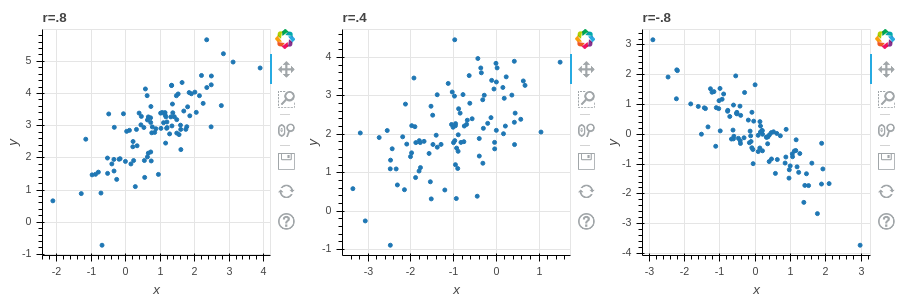
\includegraphics[width=0.5\textwidth,height=\textheight]{../img/correlation.png}
\caption{Correlation}\label{fig:corrfig}
}
\end{figure}

\hypertarget{sec:covarmat}{%
\subsubsection{The covariance matrix}\label{sec:covarmat}}

In a typical situation we have many features for each of our (many)
samples, that we organize into a data matrix \(X\). To recall, each
column of \(X\) corresponds to a feature that we measure, and each row
corresponds to a sample. For example, each row of our matrix might
correspond to a person enrolled in a study, and the columns correspond
to height (cm), weight (kg), systolic blood pressure, and age (in
years):

\begin{longtable}[]{@{}lrrrr@{}}
\caption{A sample data matrix \(X\) \label{tbl:data}}\tabularnewline
\toprule
sample & Ht & Wgt & Bp & Age\tabularnewline
\midrule
\endfirsthead
\toprule
sample & Ht & Wgt & Bp & Age\tabularnewline
\midrule
\endhead
A & 180 & 75 & 110 & 35\tabularnewline
B & 193 & 80 & 130 & 40\tabularnewline
\ldots{} & \ldots{} & \ldots{} & \ldots{} & \ldots{}\tabularnewline
U & 150 & 92 & 105 & 55\tabularnewline
\bottomrule
\end{longtable}

If we have multiple features, as in this example, we might be interested
in the variance of each feature and all of their mutual covariances.
This ``package'' of information can be obtained ``all at once'' by
taking advantage of some matrix algebra.

\textbf{Definition:} Let \(X\) be a \(k\times N\) data matrix, where the
\(N\) columns of \(X\) correspond to different features and the \(k\)
rows to different samples. Let \(X_{0}\) be the centered version of this
data matrix, obtained by subtracting the mean \(\mu_{i}\) of column
\(i\) from all the entries \(x_{si}\) in that column. Then the
\(N\times N\) symmetric matrix

\[
D_{0} = \frac{1}{N}X_{0}^{\intercal}X_{0}
\]

is called the (sample) covariance matrix for the data.

\textbf{Proposition:} The diagonal entries \(d_{ii}\) of \(D_{0}\) are
the variances of the columns of \(X\):

\[
d_{ii} = \sigma_{i}^2 = \frac{1}{N}\sum_{s=1}^{k}(x_{si}-\mu_i)^2
\]

and the off-diagonal entries \(d_{ij} = d_{ji}\) are the covariances of
the \(i^{th}\) and \(j^{th}\) columns of \(X\):

\[
d_{ij} = \sigma_{ij} = \frac{1}{N}\sum_{s=1}^{k}(x_{si}-\mu_{i})(x_{sj}-\mu_{j})
\]

\textbf{Proof:} This follows from the definitions, but it's worth
checking the details, which we leave as an exercise.

\hypertarget{linear-combinations-of-features-scores}{%
\subsubsection{Linear Combinations of Features
(Scores)}\label{linear-combinations-of-features-scores}}

Sometimes useful information about our data can be revealed if we
combine different measurements together to obtain a ``hybrid'' measure
that captures something interesting. For example, in the Auto MPG
dataset that we studied in the section on Linear Regression, we looked
at the influence of both vehicle weight \(w\) and engine displacement
\(e\) on gas mileage; perhaps their is some value in considering a
hybrid ``score'' defined as \[
S = a*w + b*e
\] for some constants \(a\) and \(b\) -- maybe by choosing a good
combination we could find a better predictor of gas mileage than using
one or the other of the features individually.

As another example, suppose we are interested in the impact of the
nutritional content of food on weight gain in a study. We know that both
calorie content and the level dietary fiber contribute to the weight
gain of participants eating this particular food; maybe there is some
kind of combined ``calorie/fiber'' score we could introduce that
captures the impact of that food better.

\textbf{Definition:} Let \(X_{0}\) be a (centered) \(k\times N\) data
matrix giving information about \(N\) features for each of \(k\)
samples. A linear synthetic feature, or a linear score, is a linear
combination of the \(N\) features. The linear score is defined by
constants \(a_{1},\ldots, a_{n}\) so that If \(y_{1},\ldots, y_{N}\) are
the values of the features for a particular sample, then the linear
score for that sample is

\[
S = a_{1}y_{1}+a_{2}y_{2}+\cdots+a_{N}y_{N}
\]

\textbf{Lemma:} The values of the linear score for each of the \(k\)
samples can be calculated as

\begin{equation}
\left[\begin{matrix} S_{1} \\ \vdots \\ S_{k}\\ \end{matrix}\right] =
X_{0}\left[
\begin{matrix} a_{1} \\ \vdots \\ a_{N}\end{matrix}\right].
\label{eq:linearscore}\end{equation}

\textbf{Proof:} Multiplying a matrix by a column vector computes a
linear combination of the columns -- that's what this lemma says.
Exercise 3 asks you to write out the indices and make sure you believe
this.

\hypertarget{mean-and-variance-of-scores}{%
\subsubsection{Mean and variance of
scores}\label{mean-and-variance-of-scores}}

When we combine features to make a hybrid score, we assume that the
features were centered to begin with, so that each features has mean
zero. As a result, the mean of the hybrid features is again zero.

\textbf{Lemma:} A linear combination of features with mean zero again
has mean zero.

\textbf{Proof:} Let \(S_{i}\) be the score for the \(i^{th}\) sample, so
\[
S_{i} = \sum_{j=1}^{N} x_{ij}a_{j}.
\] where \(X_{0}\) has entries \(x_{ij}\). Then the mean value of the
score is \[
\mu_{S} = \frac{1}{k}\sum_{i=1}^{k} S_{i} = \frac{1}{k}\sum_{i=1}^{k}\sum_{j=1}^{N} x_{ij}a_{j}.
\] Reversing the order of the sum yields \[
\mu_{S} = \frac{1}{k}\sum_{j=1}^{N}\sum_{i=1}^{k} x_{ij}a_{j} = \sum_{j=1}^{N} a_{j}\frac{1}{k}(\sum_{i=1}^{k} x_{ij})=
\sum_{j=1}^{N}a_{j}\mu_{j}=0
\] where \(\mu_{j}=0\) is the mean of the \(j^{th}\) feature (column) of
\(X_{0}\).

\textbf{Exercises.}

\begin{enumerate}
\def\labelenumi{\arabic{enumi}.}
\item
  Prove that the two expressions for \(\sigma_{X}^2\) given in
  \cref{variance} are the same.
\item
  Prove that the covariance matrix is as described in the proposition in
  \ref{sec:covarmat}.
\item
  Let \(X_{0}\) be a \(k\times N\) matrix with entries \(x_{ij}\) for
  \(1\le i\le k\) and \(1\le j\le N\). If a linear score is defined by
  the constants \(a_{1},\ldots a_{N}\), check that equation
  \cref{eq:linearscore} holds as claimed.
\end{enumerate}

The variance is more interesting, and gives us an opportunity to put the
covariance matrix to work. Remember from \ref{variance} that, since a
score \(S\) has mean zero, it's variance is \(\sigma_{S}^2=S\cdot S\) --
where here the score \(S\) is represented by the column vector with
entries \(S_{1},\ldots S_{k}\) as in \ref{eq:linearscore}.

\end{document}
